\subsubsection{Descripción y grafo de relación entre los nodos}

Para nuestro último experimento, capturamos el tráfico de la LAN de un integrante de nuestro grupo. Medimos el Miércoles 17 de Septiembre a las 00:00 utilizando la red Wi-Fi. El tiempo de medición fue de aproximadamente 40 minutos, y capturamos aproximadamente 20 paquetes.

\begin{figure}[H]
  \begin{center}
    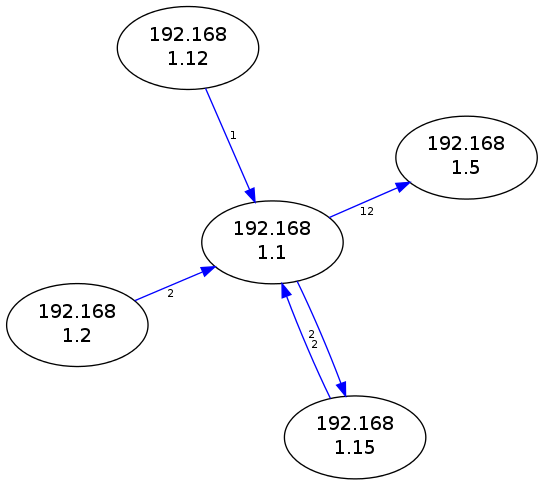
\includegraphics[width=0.3\linewidth]{../imgs/red-hogarena_red.png}
    \label{fig:FedeGrafo}
    \caption{Grafo de LAN hogareña}
  \end{center}
\end{figure}

\subsubsection{Fuente: $S_{dst}$}

\begin{figure}[H]\centering
    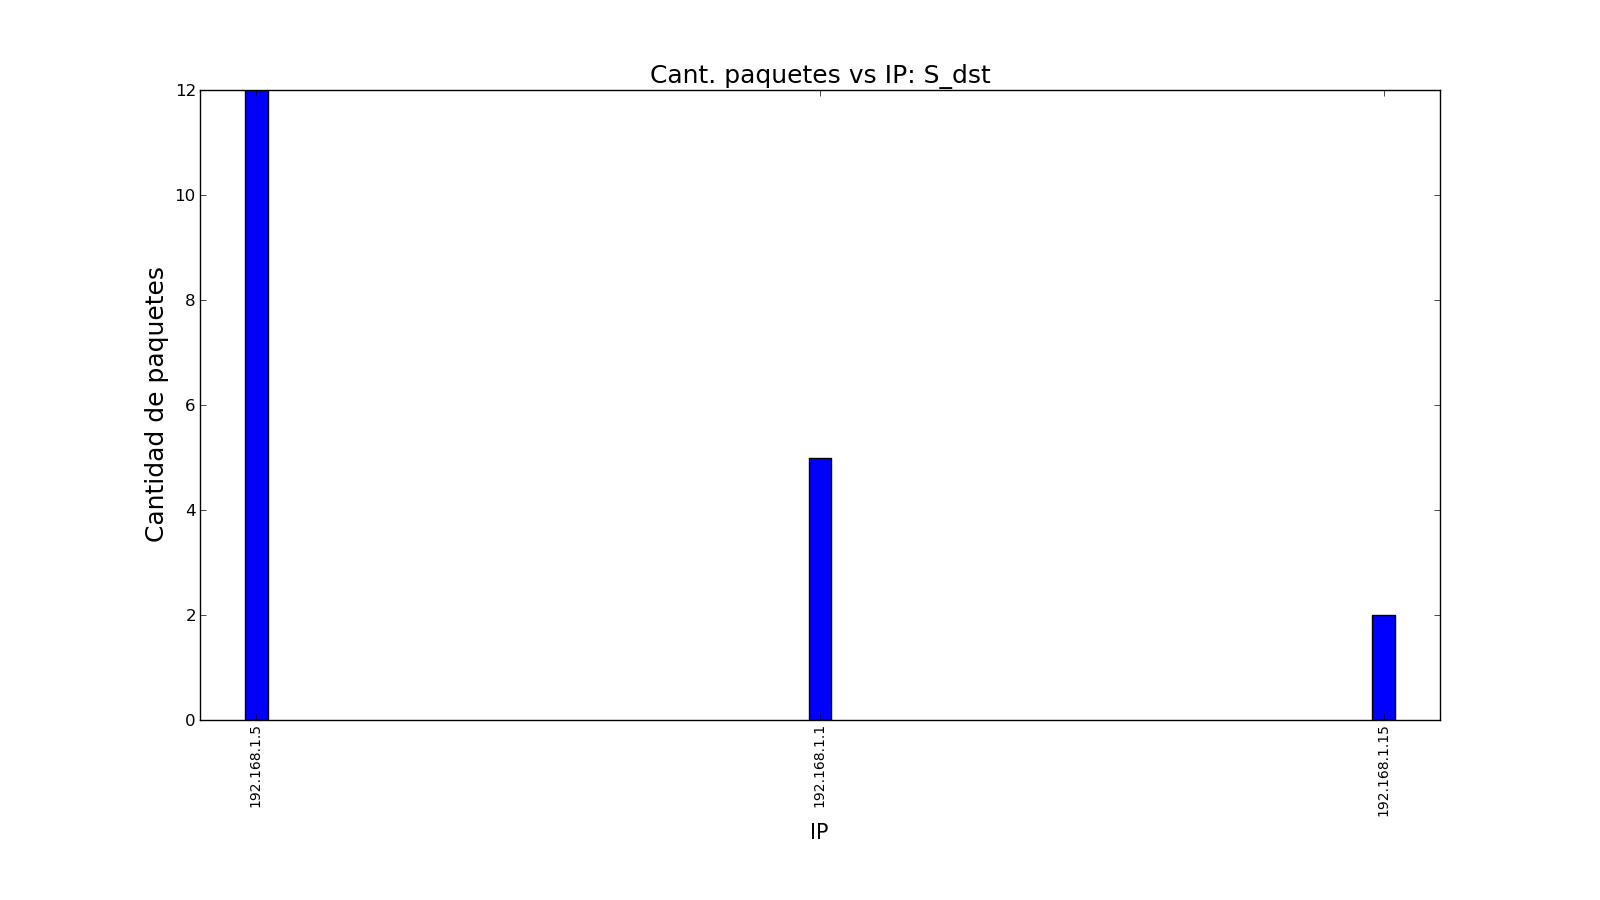
\includegraphics[width=0.8\linewidth]{../imgs/red-hogarena_S_dst_hist.png}
    \caption{Histograma de $S_{dst}$}\label{fig:Fede-dst-hist}
\end{figure}

\begin{figure}[H]\centering
    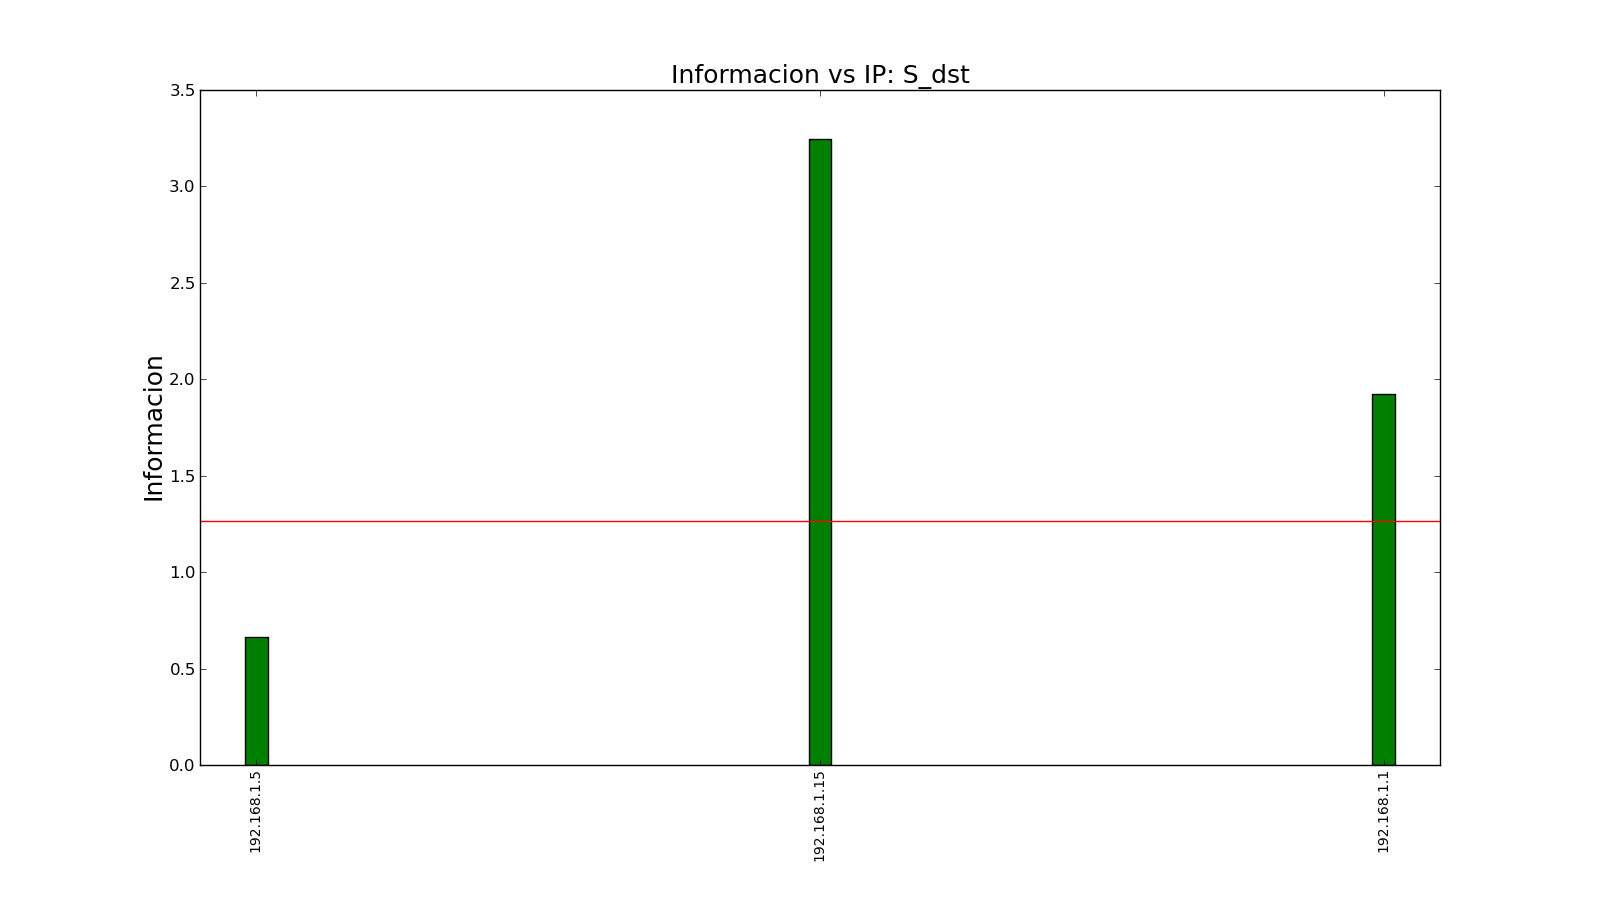
\includegraphics[width=0.8\linewidth]{../imgs/red-hogarena_S_dst_info.png}
    \caption{Informacion de $S_{dst}$}\label{fig:Fede-dst-info}
\end{figure}

$\bullet$ Entropía de la fuente: 1.26744380381

\subsubsection{Fuente: $S_{src}$}

\begin{figure}[H]\centering
    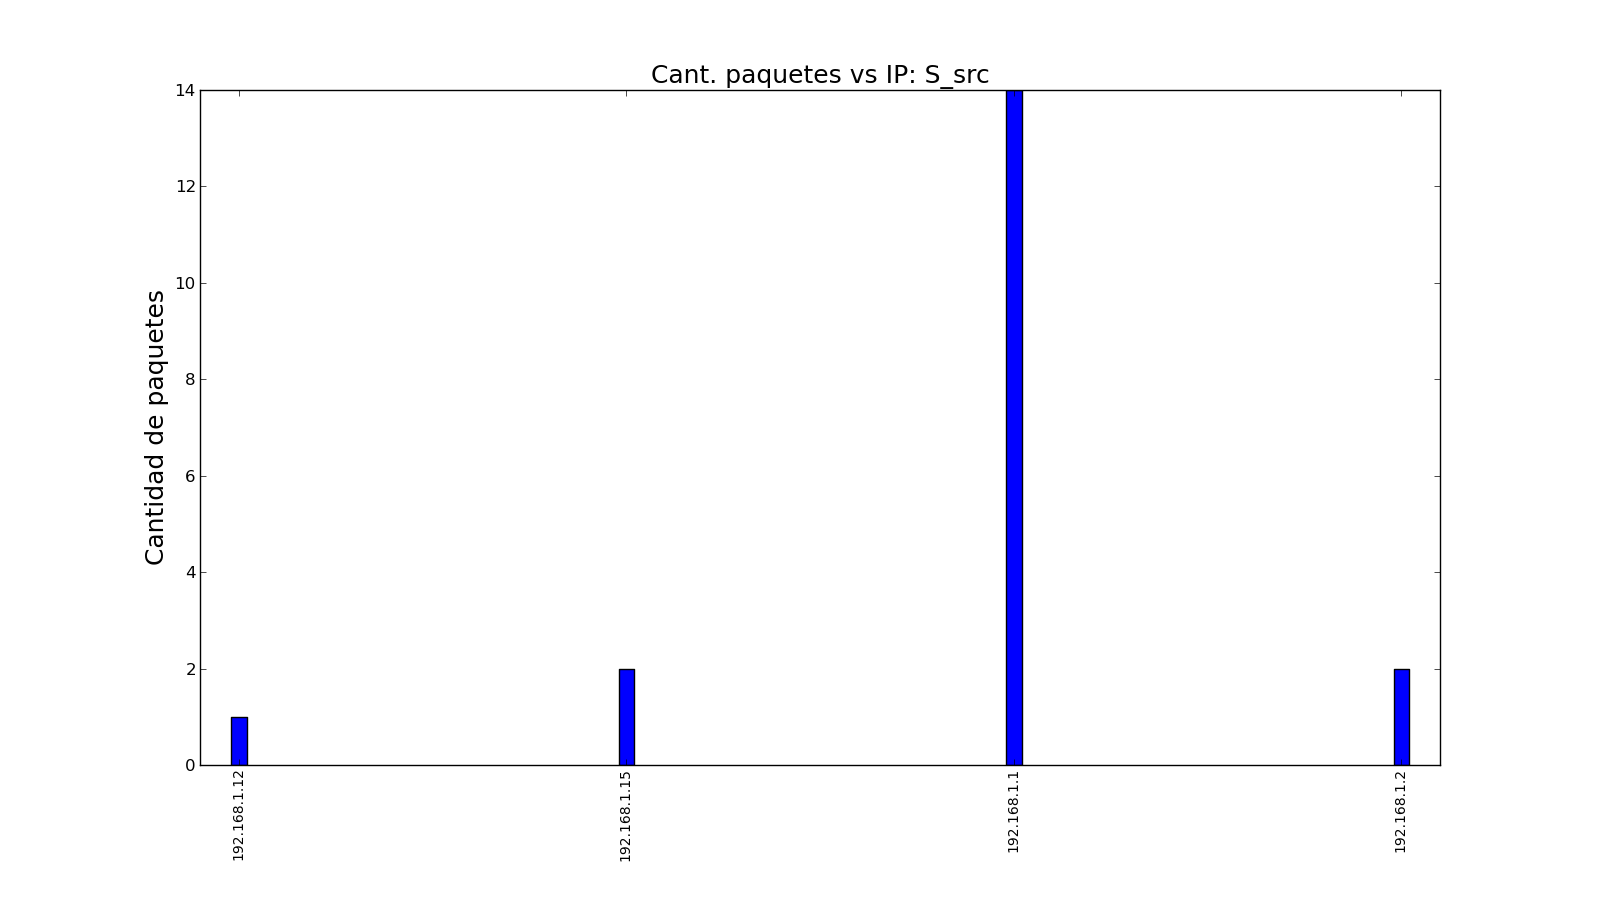
\includegraphics[width=0.8\linewidth]{../imgs/red-hogarena_S_src_hist.png}
    \caption{Histograma de $S_{src}$}\label{fig:Fede-src-hist}
\end{figure}

\begin{figure}[H]\centering
    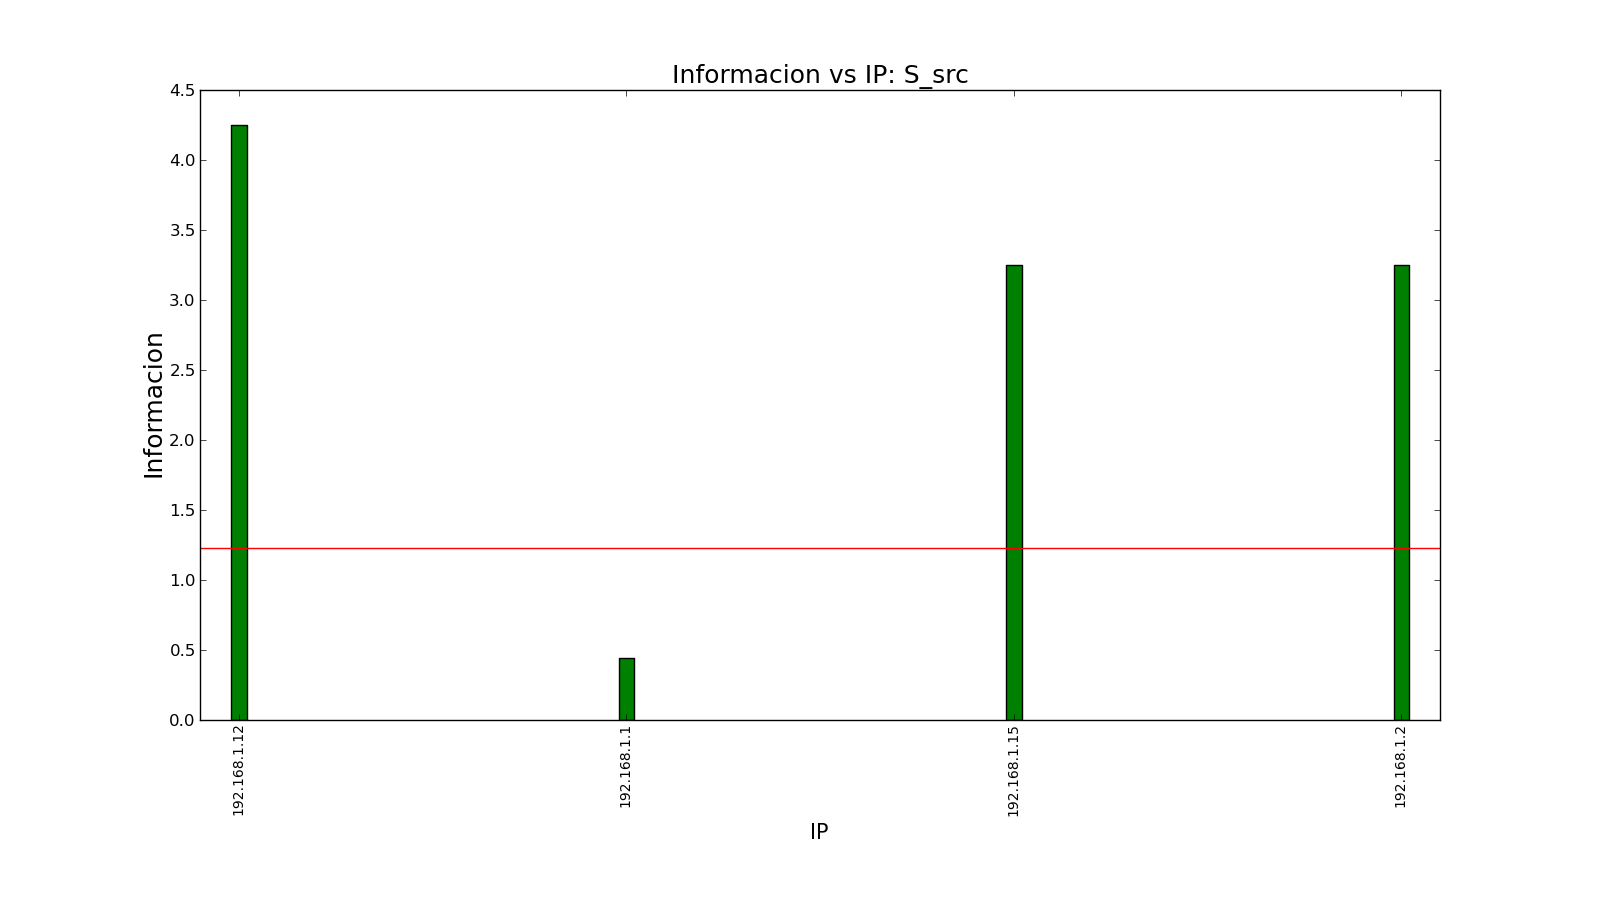
\includegraphics[width=0.8\linewidth]{../imgs/red-hogarena_S_src_info.png}
    \caption{Informacion de $S_{src}$}\label{fig:Fede-src-info}
\end{figure}

$\bullet$ Entropía de la fuente: 1.2319817814

\subsubsection{Discusión}

En este último experimento, nos encontramos con una red más chica que los otras. Esto era esperable, debido a que es una red hogareña. En el grafo podemos observar un nodo (192.168.1.1) el cual se conecta con todos los demás. Esta red la conocemos, y sabemos que dicho nodo es el router.

Como podemos observar en la Figura \ref{fig:Fede-src-info}, el router es un nodo distinguido en la fuente $S_{src}$. Sin embargo, en la Figura \ref{fig:Fede-dst-info} (fuente $S_{dst}$) el único nodo distinguido es 192.168.1.5. En el caso de 192.168.1.5, es una computadora que estaba bajando un archivo .torrent, y creemos que por eso 12 paquetes ARP \emph{who-has} tienen destino 192.168.1.5.